\FloatBarrier
\begin{figure}[!htpd]
		\centering
		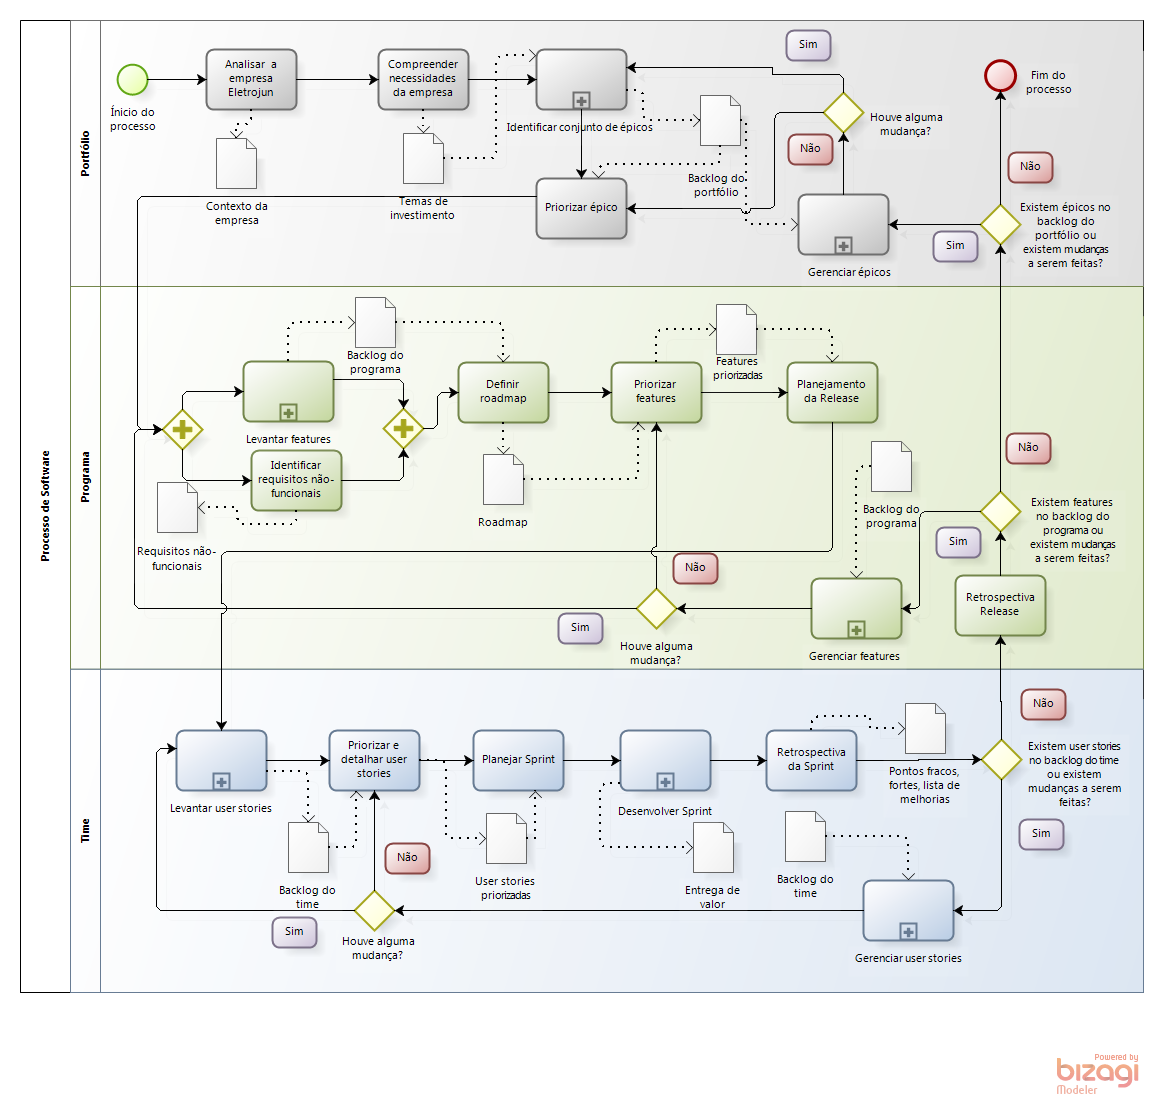
\includegraphics[scale=0.55]{figuras/Eletrojun}
		\label{img:processoeletrojun}
		\caption{Visão geral do processo para o projeto da Eletrojun}
\end{figure}
\FloatBarrier

\section {Subprocessos}

\FloatBarrier
\begin{figure}[!htpd]
		\centering
		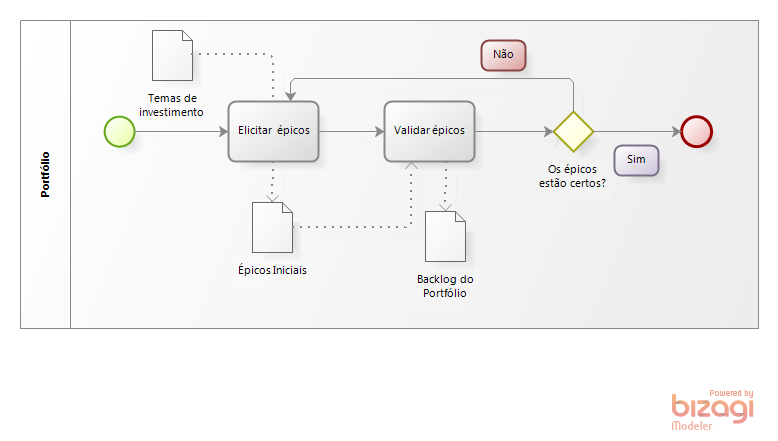
\includegraphics[scale=0.7]{figuras/epicosPRI}
		\label{img:time}
		\caption{Identificar conjunto de Épicos}
\end{figure}
\FloatBarrier

\FloatBarrier
\begin{figure}[!htpd]
		\centering
		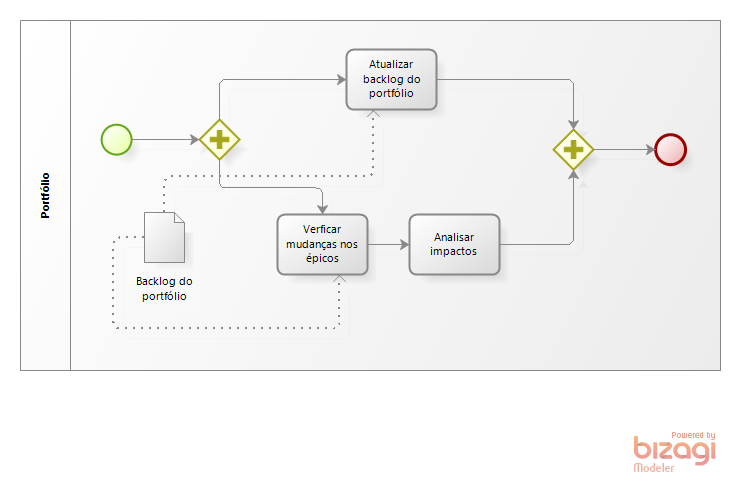
\includegraphics[scale=0.7]{figuras/epicosGRE}
		\label{img:time}
		\caption{Gerenciar Épicos}
\end{figure}
\FloatBarrier

\FloatBarrier
\begin{figure}[!htpd]
		\centering
		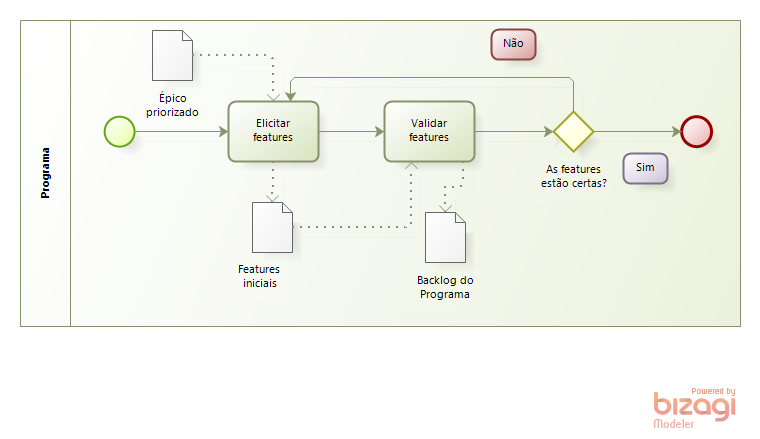
\includegraphics[scale=0.7]{figuras/FeaturesPRI}
		\label{img:time}
		\caption{Levantar Features}
\end{figure}
\FloatBarrier

\FloatBarrier
\begin{figure}[!htpd]
		\centering
		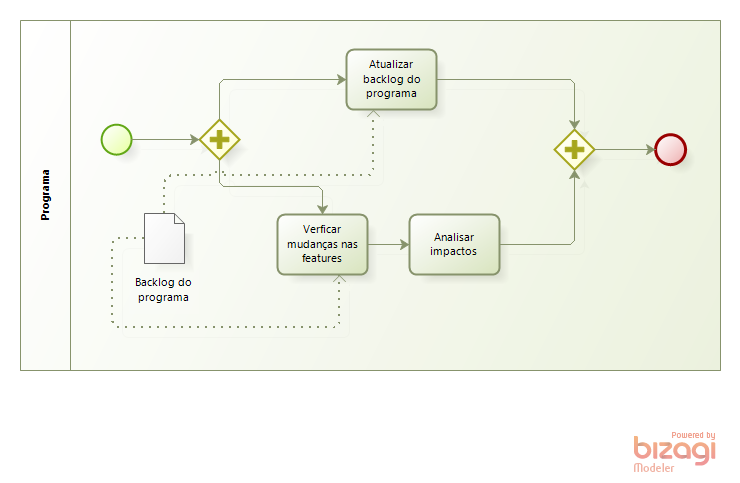
\includegraphics[scale=0.7]{figuras/featureGRE}
		\label{img:time}
		\caption{Gerenciar Features}
\end{figure}
\FloatBarrier

\FloatBarrier
\begin{figure}[!htpd]
		\centering
		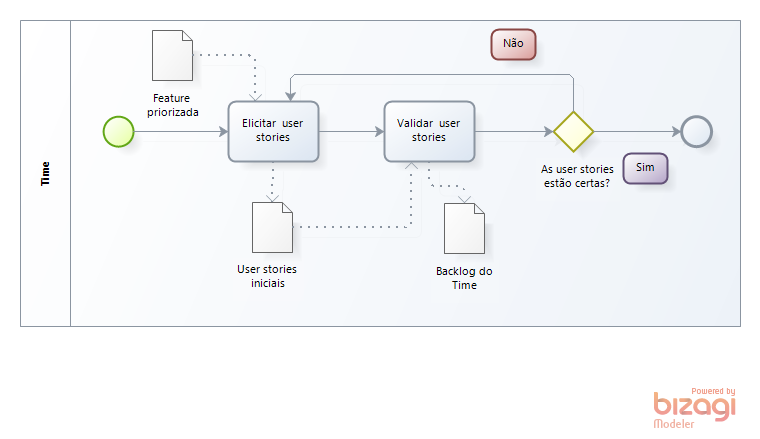
\includegraphics[scale=0.7]{figuras/usPRI}
		\label{img:time}
		\caption{Levantar User Stories}
\end{figure}
\FloatBarrier

\FloatBarrier
\begin{figure}[!htpd]
		\centering
		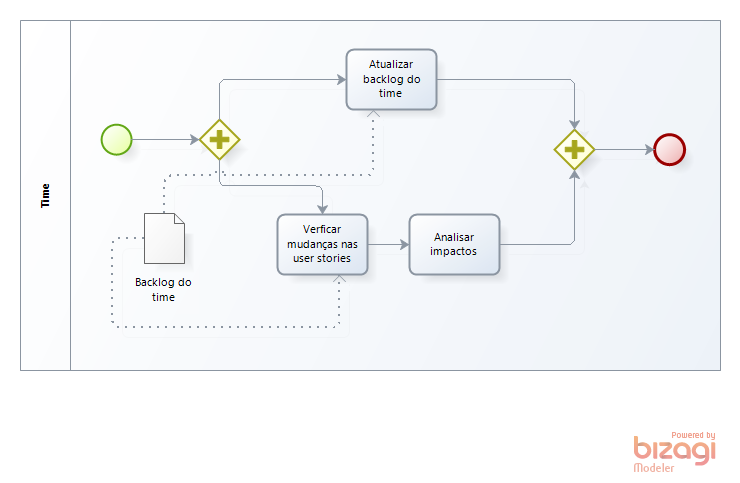
\includegraphics[scale=0.7]{figuras/usGRE}
		\label{img:time}
		\caption{Gerenciar User Stories}
\end{figure}
\FloatBarrier

\section {Portifólio}

Nesta fase, todo o esforço encontra-se diretamente relacionado ao nível de negócio. Procura-se compreender o contexto do cliente, obter o conhecimento inicial do problema, identificar características e diretrizes que posteriormente  resultarão no levantamento dos Épicos.  Estes resultados serão obtidos através da efetivação das seguintes tarefas:

\begin{itemize}
\item Analisar a empresa Eletrojun
\item Compreender necessidades da empresa
\item Identificar conjunto de Épicos
\item Priorizar Épico
\item Gerenciar Épico
\end{itemize}

\begin{table}[\htp]
\centering
\caption{Atividade 1}
\label{my-label}
\begin{tabular}{|l|l|}
\hline
ID       & 01                                                  \\ \hline
Nome     & Analisar a empresa Eletrojun.                       \\ \hline
Objetivo & Levantar informações sobre a empresa e seu negócio. \\ \hline
Entrada  &                                                     \\ \hline
Saída    & Informações sobre o contexto da empresa.            \\ \hline
\end{tabular}
\end{table}

\begin{table}[\htp]
\centering
\caption{Atividade 2}
\label{my-label}
\begin{tabular}{|l|l|l}
\cline{1-2}
ID       & 02                                                                                                                       &  \\ \cline{1-2}
Nome     & Compreender as necessidades da empresa.                                                                                  &  \\ \cline{1-2}
Objetivo & \begin{tabular}[c]{@{}l@{}}Realizar entrevista com o cliente no intuito de levantar \\ necessidades gerais.\end{tabular} &  \\ \cline{1-2}
Entrada  & Contexto da empresa.                                                                                                     &  \\ \cline{1-2}
Saída    & Contexto da empresa.                                                                                                     &  \\ \cline{1-2}
\end{tabular}
\end{table}

\begin{table}[\htp]
\centering
\caption{Atividade 3}
\label{my-label}
\begin{tabular}{|l|l|l}
\cline{1-2}
ID       & 03                                                                                                                       &  \\ \cline{1-2}
Nome     & Identificar conjunto de Épicos.                                                                                          &  \\ \cline{1-2}
Objetivo & \begin{tabular}[c]{@{}l@{}}Levantar conjunto de Épicos, analisando e estudando \\ os temas de investimento.\end{tabular} &  \\ \cline{1-2}
Entrada  & Temas de investimento.                                                                                                   &  \\ \cline{1-2}
Saída    & Backlog do portifólio.                                                                                                   &  \\ \cline{1-2}
\end{tabular}
\end{table}


\begin{table}[\htp]
\centering
\caption{Atividade 4}
\label{my-label}
\begin{tabular}{|l|l|l}
\cline{1-2}
ID       & 04                                                                                                                                   &  \\ \cline{1-2}
Nome     & Priorizar Épico.                                                                                                                     &  \\ \cline{1-2}
Objetivo & \begin{tabular}[c]{@{}l@{}}Selecionar Épico dentre o Backlog de portifólio \\ e dar preferência ao seu desenvolvimento.\end{tabular} &  \\ \cline{1-2}
Entrada  & Temas de investimento.                                                                                                               &  \\ \cline{1-2}
Saída    & Backlog do portifólio.                                                                                                               &  \\ \cline{1-2}
\end{tabular}
\end{table}


\FloatBarrier
\begin{figure}[!htpd]
		\centering
		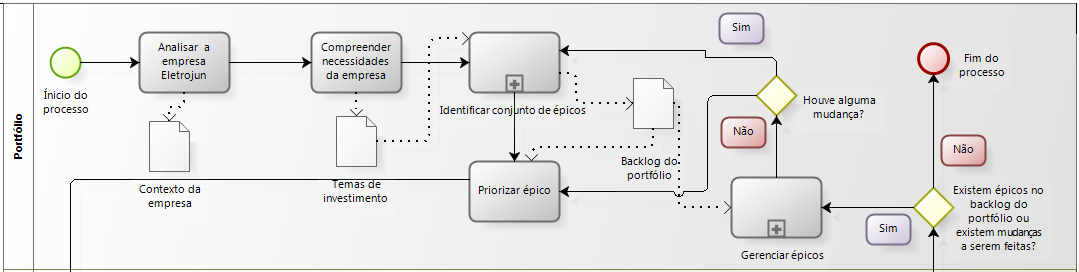
\includegraphics[scale=0.5]{figuras/Portifolio}
		\label{img:portifolio}
		\caption{Visão geral do nível de Portifólio}
\end{figure}
\FloatBarrier

\section{Programa}

Na fase de programa, o principal objetivo encontra-se em estabelecer estratégias para elaboração da solução a ser implementada, a partir da obtenção de requisitos que atendam aos sete parâmetros de qualidade (Apendice x). Estes resultados serão obtidos através da efetivação das seguintes tarefas:

\begin{itemize}
\item Levantar Feature
\item Identificar requisitos não-funcionais
\item Definir Roadmap
\item Priorizar Features
\item Planejamento da Release
\item Gerenciar Features
zitem Planejamento da Release
\end{itemize}


\begin{table}[\htp]
\centering
\caption{Atividade 5}
\label{my-label}
\begin{tabular}{|l|l|lll}
\cline{1-2}
ID       & 05                                                                                                                                        &  &  &  \\ \cline{1-2}
Nome     & Levantar Features                                                                                                                         &  &  &  \\ \cline{1-2}
Objetivo & \begin{tabular}[c]{@{}l@{}}Levantar conjunto de Features dentre o Backlog \\ de portifólio e elaborar o Backlog de programa.\end{tabular} &  &  &  \\ \cline{1-2}
Entrada  & Backlog do portifólio                                                                                                                     &  &  &  \\ \cline{1-2}
Saída    & Backlog do programa                                                                                                                       &  &  &  \\ \cline{1-2}
\end{tabular}
\end{table}


\begin{table}[\htp]
\centering
\caption{Atividade 6}
\label{my-label}
\begin{tabular}{|l|l|l}
\cline{1-2}
ID       & 06                                                                                                          &  \\ \cline{1-2}
Nome     & Definir Roadmap.                                                                                            &  \\ \cline{1-2}
Objetivo & \begin{tabular}[c]{@{}l@{}}Planejar as entregas/releases a partir da elaboração\\  do Roadmap.\end{tabular} &  \\ \cline{1-2}
Entrada  & Backlog do programa.                                                                                        &  \\ \cline{1-2}
Saída    & Roadmap.                                                                                                    &  \\ \cline{1-2}
\end{tabular}
\end{table}

\begin{table}[\htp]
\centering
\caption{Atividade 7}
\label{my-label}
\begin{tabular}{|l|l|l}
\cline{1-2}
ID       & 07                                                                                                                                                                   &  \\ \cline{1-2}
Nome     & Priorizar Features                                                                                                                                                   &  \\ \cline{1-2}
Objetivo & \begin{tabular}[c]{@{}l@{}}Selecionar Features dentre o Backlog de \\ programa, a partir de uma análise do Roadmap, \\ fazer a priorização de Features.\end{tabular} &  \\ \cline{1-2}
Entrada  & Roadmap, Backlog de programa.                                                                                                                                        &  \\ \cline{1-2}
Saída    & Features priorizadas.                                                                                                                                                &  \\ \cline{1-2}
\end{tabular}
\end{table}


\begin{table}[\htp]
\centering
\caption{Atividade 8}
\label{my-label}
\begin{tabular}{|l|l|l}
\cline{1-2}
ID       & 08                                                                                                           &  \\ \cline{1-2}
Nome     & Planejamento da Release.                                                                                     &  \\ \cline{1-2}
Objetivo & \begin{tabular}[c]{@{}l@{}}Realizar o planejamento para a release, definir os \\ pontos chaves.\end{tabular} &  \\ \cline{1-2}
Entrada  & Features priorizadas.                                                                                        &  \\ \cline{1-2}
Saída    &                                                                                                              &  \\ \cline{1-2}
\end{tabular}
\end{table}

\FloatBarrier
\begin{figure}[!htpd]
		\centering
		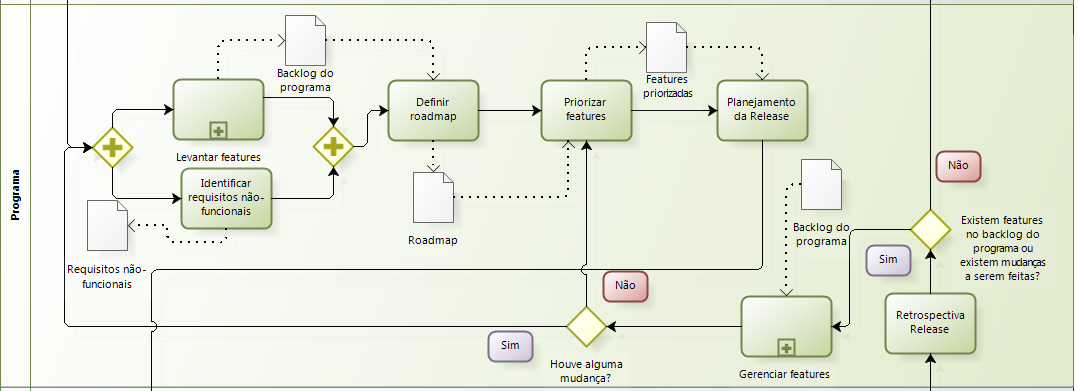
\includegraphics[scale=0.5]{figuras/Programa}
		\label{img:programa}
		\caption{Visão geral do nível de Programa}
\end{figure}
\FloatBarrier



\section{Time}

O nível Time abrange as tarefas a nível de implementação. Seu principal objetivo encontra-se no planejamento e implementação das funcionalidades definidas nas User Stories.  Estes resultados serão obtidos através da efetivação das seguintes tarefas:

\begin{itemize}
\item Levantar User Stories
\item Priorizar e detalhar User Stories
\item Planejar Sprints
\item Desenvolver Sprints
\item Retrospectiva da Sprint
\item Gerenciar User Stories
\end{itemize}


\begin{table}[\htp]
\centering
\caption{Atividade 9}
\label{my-label}
\begin{tabular}{|l|l|l}
\cline{1-2}
ID       & 09                                                                                                                                &  \\ \cline{1-2}
Nome     & Levantar user stories.                                                                                                            &  \\ \cline{1-2}
Objetivo & \begin{tabular}[c]{@{}l@{}}Realizar o levantamento das histórias de usuário e\\ com isso elaborar o backlog do time.\end{tabular} &  \\ \cline{1-2}
Entrada  & Features priorizadas.                                                                                                             &  \\ \cline{1-2}
Saída    & Backlog do time.                                                                                                                  &  \\ \cline{1-2}
\end{tabular}
\end{table}

\begin{table}[\htp]
\centering
\caption{Atividade 10}
\label{my-label}
\begin{tabular}{|l|l|l}
\cline{1-2}
ID       & 10                                                                                                                            &  \\ \cline{1-2}
Nome     & Planejar Sprint.                                                                                                              &  \\ \cline{1-2}
Objetivo & \begin{tabular}[c]{@{}l@{}}Realizar o planejamento da sprint a ser desenvolvida,\\ definir e distribuir tarefas.\end{tabular} &  \\ \cline{1-2}
Entrada  & Backlog do time com User Stories priorizadas.                                                                                 &  \\ \cline{1-2}
Saída    & Kanban atualizado.                                                                                                            &  \\ \cline{1-2}
\end{tabular}
\end{table}

\begin{table}[\htp]
\centering
\caption{Atividade 11}
\label{my-label}
\begin{tabular}{|l|l|}
\hline
ID       & 11                                            \\ \hline
Nome     & Desenvolver Sprint. \\ \hline
Objetivo & Executar Sprint, desenvolvendo as user stories.
 \\ \hline
Entrada  & Backlog do time atualizado, kanban. \\ \hline
Saída    &  Entrega de Valor.\\ \hline
\end{tabular}
\end{table}


\begin{table}[\htp]
\centering
\caption{Atividade 12}
\label{my-label}
\begin{tabular}{|l|l|l}
\cline{1-2}
ID       & 12                                                                                                                                          &  \\ \cline{1-2}
Nome     & Retrospectiva da Sprint.                                                                                                                    &  \\ \cline{1-2}
Objetivo & \begin{tabular}[c]{@{}l@{}}Realizar reunião de retrospectiva da Sprint, de modo\\ a discutir os pontos positivos e negativos.\end{tabular}  &  \\ \cline{1-2}
Entrada  &                                                                                                                                             &  \\ \cline{1-2}
Saída    & \begin{tabular}[c]{@{}l@{}}Lista de melhorias a serem implementadas, pontos \\ fortes e fracos da sprint, aspectos a melhorar.\end{tabular} &  \\ \cline{1-2}
\end{tabular}
\end{table}

\FloatBarrier
\begin{figure}[!htpd]
		\centering
		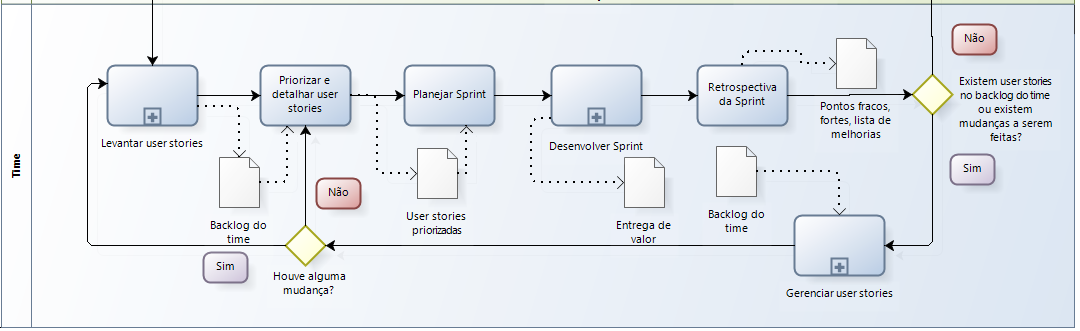
\includegraphics[scale=0.5]{figuras/Time}
		\label{img:time}
		\caption{Visão geral do nível de Time}
\end{figure}
\FloatBarrier

\section{Relação Entre Atividades e Modelo de Maturidade MPS.BR}

Baseado no Modelo de Maturidade adotado no projeto, o MPS.BR, as atividades descritas acima foram concebidas de forma a atender os resultados esperados referentes às atividades de Engenharia de Requisitos presentes nos níveis D e G do modelo.

	O mapeamento entre atividade e resultado esperado é descrito a seguir:

\subsection{Atividades}

\textbf{ Nível de Portifólio:}

\begin{enumerate}
\item P01 - Analisar a empresa Eletrojun.
\item P02 - Compreender as necessidades da empresa.
\item P03 - Identificar conjunto de épicos.
\item P04 - Priorizar épico.
\item P05 - Gerenciar épicos
\end{enumerate}

\textbf{Nível de Programa:}

\begin{enumerate}
\item R01 - Levantar features.
\item R02 - Identificar requisitos não-funcionais
\item R03 - Definir roadmap.
\item R04 - Priorizar features.
\item R05 - Planejamento da release.
\item R06 - Gerenciar features
\item R07 - Retrospectiva da release
\end{enumerate}

\textbf{ Nível de Time:}

\begin{enumerate}
\item T01 - Levantar user stories.
\item T02 - Priorizar e detalhar user stories.
\item T03 - Planejar sprint.
\item T04 - Desenvolver sprint.
\item T05 - Retrospectiva da sprint.
\item T06 - Gerenciar user stories.
\end{enumerate}

\subsection{Resultados Esperados}

\textbf{Nível G}

\begin{enumerate}
\item GRE 1 - Comunicação constante com os fornecedores de requisitos;
\item GRE 2 - Os requisitos são compreendidos;
\item GRE 3 - Requisitos são aceitos;
\item GRE 4 - Comprometimento com os requisitos;
\item GRE 5 - Rastreabilidade entre os requisitos, planos do projeto e produtos do trabalho;
\item GRE 6 - São corrigidas as inconsistências entre os requisitos, planos e produtos do projeto;
\item GRE 7 - Ao longo do projeto as mudanças nos requisitos são gerenciadas.
\end{enumerate}

\textbf{Nível D}

\begin{enumerate}
\item DRE 1 - São identificadas as necessidades, expectativas, restrições e requisitos de interface do cliente;
\item DRE 2 - Requisitos funcionais e não-funcionais são estabelecidos;
\item DRE 3 - Requisitos são refinados;
\item DRE 4 - Conceitos operacionais e cenários são desenvolvidos;
\item DRE 5 - A definição das  funcionalidades são desenvolvidas;
\item DRE 6 - Requisitos são avaliados para assegurar as necessidades dos interessados;
\item DRE 7 - Requisitos são validados.
\end{enumerate}

\subsection{Mapeamento}

\begin{table}[\htp]
\centering
\caption{Mapeamento das atividades e MPS}
\label{my-label}
\begin{tabular}{|l|l|l}
\cline{1-2}
Resultado Esperado & Atividade                                                                                       &  \\ \cline{1-2}
GRE 1              & \begin{tabular}[c]{@{}l@{}}P02, P03, P05, R01, R05, R06, R07, T01,\\ T03, T05, T07\end{tabular} &  \\ \cline{1-2}
GRE 2              & P03, P05, R01, R02, R06, T01, T06, T07                                                          &  \\ \cline{1-2}
GRE 3              & P03, P05, R01, R02, R06, T01, T06, T07                                                          &  \\ \cline{1-2}
GRE 4              & P05, R06, T06                                                                                   &  \\ \cline{1-2}
GRE 5              & R03, R05, T03                                                                                   &  \\ \cline{1-2}
GRE 6              & P05, R06, T06                                                                                   &  \\ \cline{1-2}
GRE 7              & P05, R06, T06                                                                                   &  \\ \cline{1-2}
DRE 1              & P02, P03, P05, R01, R02, R06, T01, T06                                                          &  \\ \cline{1-2}
DRE 2              & P02, P03, P05, R01, R02, R06, T01, T06                                                          &  \\ \cline{1-2}
DRE 3              & T02, T06                                                                                        &  \\ \cline{1-2}
DRE 4              & P02, P03, R01, T01                                                                              &  \\ \cline{1-2}
DRE 5              & P02, P03, P05, R01, R02, R06, T01, T06                                                          &  \\ \cline{1-2}
DRE 6              & P05, R06, T06                                                                                   &  \\ \cline{1-2}
DRE 7              & P05, R06, T06                                                                                   &  \\ \cline{1-2}
\end{tabular}
\end{table}
